\documentclass{sig-alternate}
\usepackage{graphicx, tabularx, amssymb, amsmath}
\usepackage{subfigure}
\usepackage{algorithm}
\usepackage{algpseudocode}
\usepackage{url}
\usepackage{flushend}
\usepackage{multirow}

\begin{document}

\title{Energy-Aware Synthesis of Application Specific MPSoCs }

\maketitle

\begin{abstract}

Application specifc multi-processor system on chip (MPSoC) can be used to execute streaming applications in a pipelined manner. Each processing element (PE) in the pipeline can be customized depending on the target constraints imposed by the system designer leading to an heterogenous system.
 
The processing elements can be customized by adding application-specific custom instructions set, selecting appropriate cache configurations and by setting different voltage and frequency. In this paper, we propose a framework to synthesize an heterogeneous application specific MPSoC for the target streaming application. Our framework optimizes for the total energy consumption provided the pipeline period constraint and the silicon area budget. We obtain the optimal points with an efficient branch and bound algorithm. Our results show that the optimally configured ASIP MPSoC by our method acheives significant energy reduction compared to the conventional techniques. 


%We also compare our technique with the traditional two staged approach on optimizing the %energy. Our technique acheives on an average x \% reduction in energy compared to the %conventional approaches. 


\end{abstract}

\section{Introduction}
MultiProcessor System on Chips (MPSoCs) have significantly proliferated in the embedded system domain due to the scaling of transistor. Furthermore, the MPSoCs can be configured to satisfy the requirements of the target applications, leading to an Application Specific MPSoC. The cores in Application Specific MPSoC can be diverse in nature and may include coprocessors, DSPs,  general purpose processors or hardware accelerators. The heterogeneity in designing Application Specifc MPSoC can be exploited to improve the efficiency of parameters like performance, area and energy consumption for the target application.

Low energy consumption is highly desirable for MPSoCs that are used in portable devices to increase the battery life of the device. Prior research has shown that the use of Dynamic Voltage and Frequency Scaling (DVFS) and customization of the processors are two effective techniques for reduction of energy consumption ~\cite{energy_asip}. This is particularly so for
streaming applications, which contain sub-kernels that are executed
repeatedly in a pipelined fashion~\cite{pipeline}. DVFS results in quadratic
reduction in energy with only linear sacrifice of the processor speed.
Streaming applications benefit from DVFS by exploiting the slack of non-
critical stages to reduce their dynamic energy consumption.

Customization of the processors in an MPSoC is typically achieved through
the use of Application Specific Instruction set Processors (ASIPs) ~\cite{sun_asip}.
ASIPs can be customized according to the sub-kernels of a streaming
application. The addition of custom instructions to an ASIP improves it's
energy efficiency for the following reasons: the number of instruction
fetches reduces, and the number of register file accesses for data
transfer between the instructions reduces ~\cite{energy_custom}. On the other hand,
custom instructions can also have a detrimental effect because of the
increase in on-chip area, and thus in the leakage energy consumption.
Hence, a designer has to carefully choose custom instructions to minimze
the energy consumption. 

In an ASIP, the memory subsystem (caches) contributes significantly to
its total energy consumption ~\cite{mem_en1, mem_en2}. In particular, the memory subsystem
is a significant contributor of the on-chip area, and thus of the total
leakage energy consumption. Therefore, design of a memory subsystem
is also crucial in improving not only the energy efficiency, but also
the performance and the area utilization of an ASIP. Existing works on
reducing energy consumption in the memory subsystems are~\cite{mem_en2}. 

Traditionally, researchers have focussed on reducing energy consumption
of ASIP based MPSoCs with the addition of custom instructions or
customization of the cache or the use of DVFS. They fail to consider
all the three techniques together for maximal reduction in energy
consumption. With the customization of the ASIPs and their caches, and
the added advantage of DVFS, one can synergistically design an energy-
efficient heterogeneous MPSoC for streaming applications, which are the
basis of entertainment in portable devices~\ref{}.

\begin{figure}[h]
\label{fig:motivation}
\center
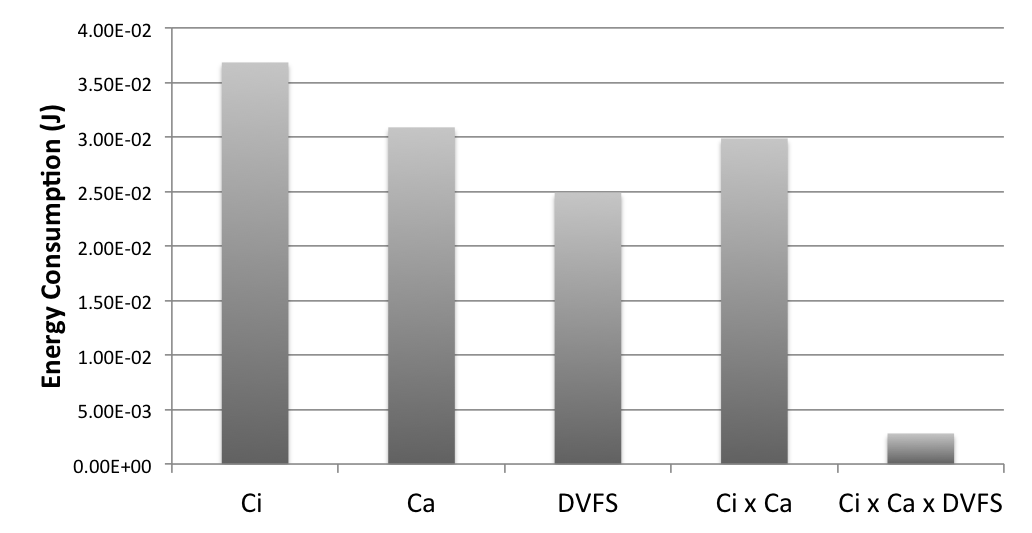
\includegraphics[width=0.40\textwidth]{motivation.png}
\caption {Minimal Energy Consumption for DCT kernel of MP3 encoder}
\end{figure}

To show the importance of considering all the three techniques
together, we analyze a sub-kernel of a streaming application. We
chose \textit{discrete cosine transform (DCT)} sub-kernel from the
\textit{MP3} encoder application. The experimental setup is described
in detail in Section~\ref{}. Figure~\ref{} plots the minimal energy
consumption achievable for each of the following techniques: a) Only custom instructions are added (\textbf{Ci}), b) Only cache
is customized (\textbf{Ca}), c) Only DVFS is used (\textbf{DVFS}
) d) Custom instructions are added with customization of the cache
(\textbf{Ci $\times$ Ca}) and e) All the three techniques are considered
simultaneously (\textbf{Ci $\times$ Ca $\times$ DVFS}). Use of both the
custom instructions and customized cache is better than their individual
use because addition of custom instructions modifies a kernel’s behaviour
such as code size, data transfers between instructions, memory access
pattern, etc. Therefore, a designer should choose an appropriate cache
based on the custom instructions to improve the energy efficiency. Next,
the use DVFS, in addition to custom instructions and customized cache,
results in minimum energy consumption, which is significantly lower than
the other techniques. Thus, it is evident that separate use of the three
energy reduction techniques may result in a local optima. Therefore, it
is desirable to use all the three techniques together to reach better
global optima.

Although the use of custom instructions, customized cache and DVFS
achieves better energy efficiency, their combined use significantly
increases the complexity of the optimization problem. For instance,
consider an application with only four tasks, four different custom
instructions per task, four different voltage/frequency levels and four
different cache configurations. Then, the total number of points in the
design space is more than a billion. Therefore, in this paper, we focus
on the problem of selecting custom instructions, cache configuration and
voltage/frequency level for sub-kernels of a streaming application, which
is executed on an MPSoC. To aid quick and efficient exploration of the
design space, first we propose estimation methods to compute execution
time and energy consumption of a sub-kernel. Then, we design a novel
branch and bound algorithm to efficiently prune and search the design
space. In particular, this paper has the following contributions:

\begin{enumerate}

\item We propose a novel problem formulation for ASIP systhesis based on
energy efficiency.

\item We develop an analytical framework to explore the complex design
space involving custom instruction set versions, cache sizes and voltage/
frequency settings simultaneously.

\item We propose a novel branch and bound algorithm to identify the
optimal points in the complex design space.

\item Finally, we compare our technique with the exisiting conventional
techniques for energy optimization.

\end{enumerate}

\section{Related Work}


%\section{Motivational Example}
\label{sec:motivation}

To show that designing an optimal memory system for energy efficiency of the entire ASIP, we analyze a kernel in a streaming application. We chose \textit{discrete cosine transform (DCT)} kernel of the streaming application \textit{MP3} encoder. The experimental setup will be described in detail in Section \ref{}. Figure \ref{fig:cis-mem} shows the core and total energy consumption of the various customized versions of \textit{DCT} for a fixed cache size. {\bf to do: define core energy and memory}. The customized versions are sorted according to the decreasing order of the execution time (i.e) the execution time of $custom_i$ < $custom_j$, if \begin{math}i<j\end{math}. It is evident from the Figure \ref{} that the total energy consumption of the system does not follow the same trend as the core energy consumption. For example, $custom_3$ has lower core energy compared to $custom_2$ but the total energy follows the other trend. Thus, an holistic approach is required in selecting appropriate custom instructions and memory subsytem in designing energy efficient ASIP system. 
\begin{figure}[h]
\center
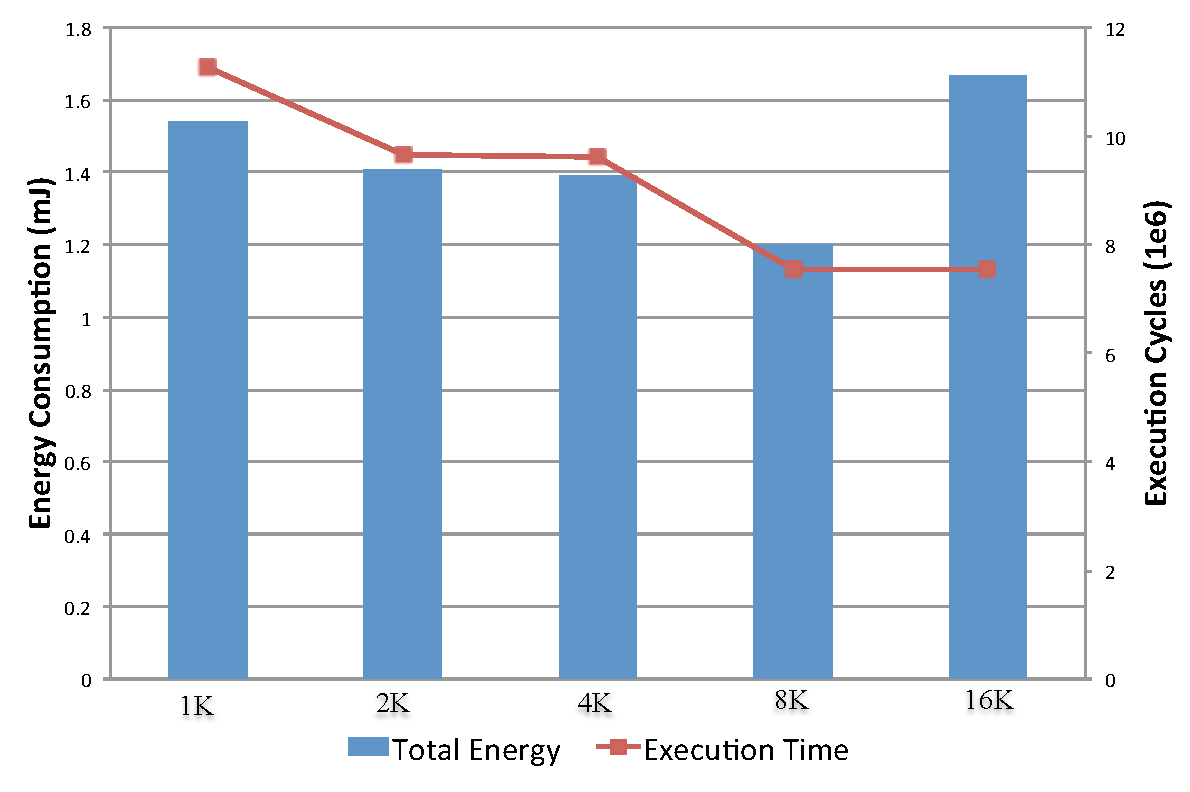
\includegraphics[width=0.36\textwidth]{cache-size.pdf}
\label{fig:cache-size}
\caption {Impact of various cache size on a particular customized version}
\end{figure}

Figure \ref{fig:cache-size} illustrates the effect of the various cache sizes of a particular customized version of \textit{DCT} on the total energy consumption and execution time. We modify the instruction cache sizes from 1KB to 16KB. In terms of performance, the most optimal cache size is 16KB. With insignificant performance loss, the optimal cache in terms of energy is 8KB. Furthermore, area saving by going from 16KB to 8KB is significant (from Table \ref{} ). It is very important for the designer to choose the appropriate cache size for the most efficient energy ASIP system. 

In our framework along with custom instruction and cache size selection, we also incorporte voltage/frequency scaling to improve the energy. Just by considering any of the techniques individially may result in a local optima. Thus, it is important to consider all the three techniques collectively to reach a global optimal point. To justify this claim, we have provided extensive results in Section \ref{sec:experiment}.  


\section{Problem Formulation}
\label{sec:problem_statement}

In this paper, we target heterogeneous MPSoCs that consist of
customizable Processing Elements (PEs), which can be realized with the
use of ASIPs. Each PE has private cache and communicates with other PEs
via dedicated communication buffers (for example, FIFO queues). Each
PE can be customized by both extending its baseline instruction set
architecture and customizing its cache. Additionally, each PE can operate
in several discrete voltage and frequency levels. Thus, the heterogeneity
in the MPSoC is manifested in terms of custom instructions, custom cache
configurations and voltage/frequency levels.

The target application domain comprises of streaming applications, which
contains multiple compute-intensive sub-kernels or tasks. The task graph
of an application is a directed acyclic graph, where the tasks are
mapped to PEs to enable pipelined execution of the streaming application. 
Figure~\ref{fig:pipeline} illustrates the pipelined execution in MPSoC. For example, two tasks are mapped to the first PE and one task is mapped to the second PE. The PEs form the logical stages of the pipeline. At the end of each stages of the pipeline, a single iteration of a task is completed. The steady state in the given example is reached after the stage one of the second PE. The period of the pipeline is defined as the maximum latency among all the stages (as shown in Figure~\ref{fig:pipeline}. 

Each task can be accelerated with a set of custom instructions. Hence, there are multiple
implementations of each task corresponding to differing sets of custom
instructions that can be used. Each set of custom instructions for a
task is associated with its additional area. Furthermore, each task can
be executed with one of the available discrete voltage and frequency
levels. The execution time and energy consumption of a task then depends
on the cache configuration of the PE on which it is mapped, and the set
of custom instructions and voltage/frequency level selected for it. The
area of the baseline PE, additional custom instructions and the cache
configuration determines the total area of the PE. The area of the
MPSoC is then the summation of the area of all the PEs.

Benoit et al.~\cite{general_mapping} categorizes the policies to map tasks of a task
graph on an MPSoC with fixed number of PEs into: one-to-one mapping,
where only a single task is mapped to a PE; interval based mapping, where
only adjoining tasks are mapped to a PE; and, general mapping, where no
restrictions are placed at all. In this paper, we use general mapping
which offers greater flexibility, and has the potential to reach better
global optima. In summary, our design space exploration should
search through: a) the number of PEs, b) mapping of the tasks on the
the PEs, c) the cache configurations for each of the PEs, d) the sets of
custom instructions for each of the tasks , and e) the voltage/frequency
levels for each of the tasks.

The problem can be formally stated as follows: given an acyclic task
graph of an application, differing sets of custom
instructions for each task, differing discrete voltage/frequency levels
for each task, differing cache configurations for a PE, the steady state
period constraint and the area constraint, the goal is to minimize the
total energy consumption of the MPSoC. Therefore, the following need to
be determined:
\begin{itemize}
\item The energy-wise optimal number of PEs and mapping of the tasks on them.
\item The energy-wise optimal cache configuration for the each of the
individual PEs.
\item The energy-wise best set of custom instructions and voltage/
frequency level for each task.
\end{itemize}

Note that the optimization problem described above cannot be solved
naively because of its exponential complexity, which results from all
the possible combinations of task mapping, cache configurations, sets of
custom instructions, and voltage/frequency levels.


\begin{figure}[h]
\center
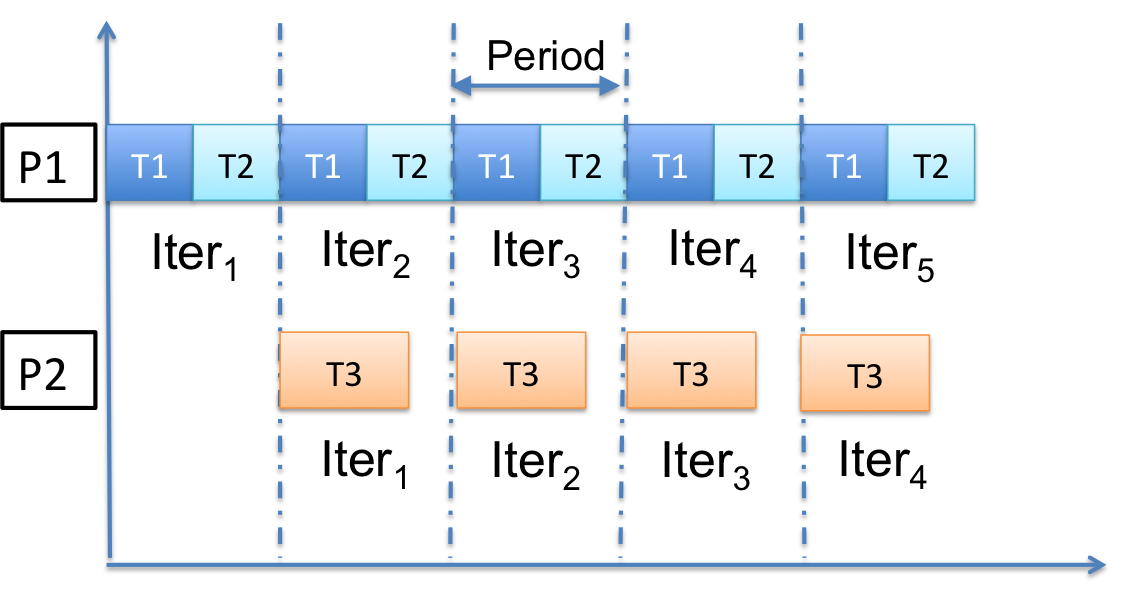
\includegraphics[scale=0.40]{pipeline.png}
\label{fig:pipeline}
\caption {Pipelined Execution}
\end{figure}


\section{Proposed Framework}
\label{sec:framework}

In this section, we explain our framework to solve the energy
optimization problem described in the last section. The input to the
framework is as follows: A streaming application, which is represented
as a task graph with N tasks $\textless T_{1}, T_{2}, ..., T_{N}
\textgreater$, $M_{i}$ sets of custom instructions for the task $T_i
\textless CI_{i1}, ..., CI_{iM}\textgreater$, V levels of available
voltages/frequencies $\textless vf_{1}, ..., vf_{V}\textgreater$ and C
cache configurations $\textless Ca_{1}, ..., Ca_{C}\textgreater$. The
designer provides the steady state \textit{period} constraint, $P_{c}
$, and the \textit{area} constraint, $A_{c}$ as the input constraints
to the framework. Figure \ref{fig:framework} shows the flow of the
framework. In the profiling stage, we profile the differing sets of
custom instructions of the individual tasks on a single PE at differing
voltage/frequency levels and with differing cache configurations to
obtain latencies and energy consumptions of their single iterations. For
instance, for task $T_{i}$, $M_{i} \times V \times C$ simulations are
run to capture latency and energy consumption of every implementation
of $T_{i}$ on a single PE. Additionally, we collect the trace of each
simulation during the profiling stage. The second stage, named latency-
energy estimation, is then used to analytically estimate the latency
and energy consumption of differing mappings of the tasks on the PEs
using the profiling information and traces generated by the first stage.
Lastly, the framework uses a novel branch and bound algorithm based upon
the estimation performed by the second stage to quickly and efficiently
prune and search the design space for the optimal design point -- the one
with minimum energy consumption.

\begin{figure}[h]
\center
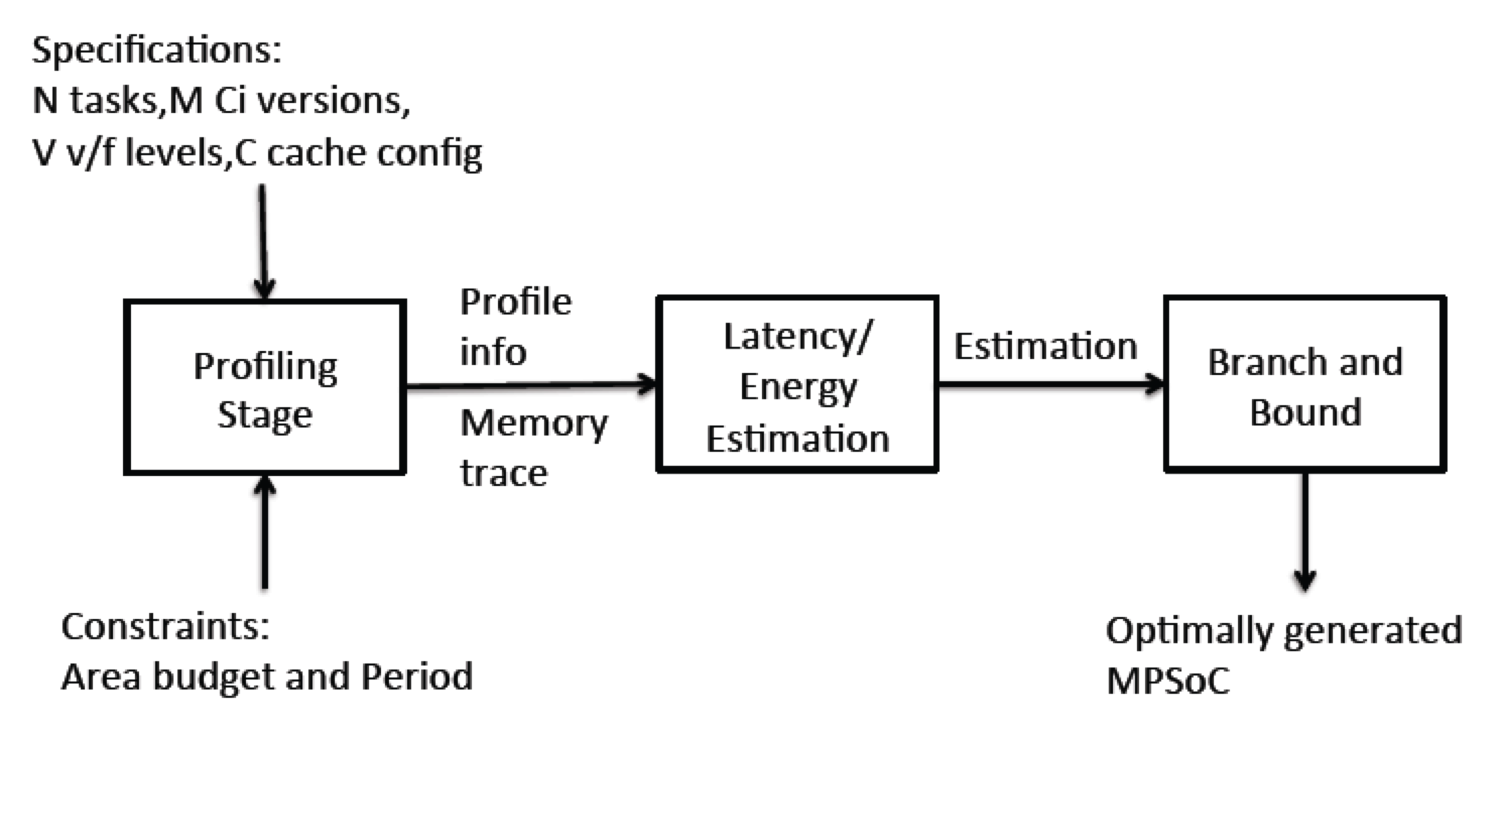
\includegraphics[width=0.40\textwidth, height=0.27\textwidth]{framework.png}
\label{fig:framework}
\caption {Framework Flow}
\end{figure}

\subsection{Latency-Energy Estimation}

As mentioned earlier, we use general task mapping as it allows greater
flexibility and efficiency in terms of energy. Generating all the possible task mappings
is equivalent to enumerating all the possible set partitions~\cite{}.
For example, an application, consisting of five tasks, can be mapped
onto five PEs in 52 different ways (some PEs might not have any task
mapped on them). It is not realistic to simulate all the possible
mappings of all the tasks when the number of tasks increases. This is
further exacerbated by the availability of differing custom instructions,
cache configurations and voltage/frequency levels. Therefore, the
\textit{profiling stage} simulated only mapping of a task on a single
PE, with its differing custom instructions, cache configurations and
voltage/frequency levels so as to keep the simulation time minimal
and reasonable. Furthermore, the simulations in the \textit{profiling
stage} were only done for a single iteration, and hence do not represent
the steady state. Now, we propose a technique to estimate the latency
and energy consumption of a task under steady state and its different
mappings.
\begin{center}
\begin{table}\scriptsize
\begin{tabular}{|c|c|c|c|}
\hline
After & Cache State (CS) & Compulsory  & Capacity/ \\
Iteration & & Misses (Comp) & Conflict Misses \\
\hline 
1 & $\lbrace m_0,m_5,m_6,m_7 \rbrace$ & $\lbrace m_0,m_1,m_2,m_3\rbrace$ & $\lbrace m_5,m_6,m_7\rbrace$ \\
\hline 
2 & $\lbrace m_0,m_5,m_6,m_7 \rbrace$ & $\boldsymbol{\lbrace m_1,m_2,m_3\rbrace}$ & $\lbrace m_5,m_6,m_7\rbrace$ \\
\hline
3 & $\lbrace m_0,m_5,m_6,m_7 \rbrace$ & $\boldsymbol{\lbrace m_1,m_2,m_3\rbrace}$ & $\lbrace m_5,m_6,m_7\rbrace$ \\
\hline
\end{tabular}
\caption{Cache across iterations}
\label{tab:c_iter}
\end{table}
\end{center}

The latency and energy consumption of a task depends on the number of cache hits/misses.  Cache misses can be broadly classified as compulsory
misses, capacity misses and conflict misses. The capacity and conflict
misses remain constant across all the iterations of a task. Thus, the capacity and conflict misses can be captured by executing a single iteration of the task, which was done in the profiling
stage. In the steady state, the compulsory misses change across iterations which is due to the repeated execution of the task. Consider that the terminology "cache state" denotes the contents of all the cache blocks for a given cache configuration. For the sake of
simplicity, a direct mapped cache is assumed in the following example.
However, the estimation technique can easily be extended to set-
associative caches. The state of a direct mapped cache is a set of n
elements, c[0 ... n-1], where c[i] = m if the cache block i holds the
memory block m. Let $Comp$ be the set representing the blocks that were fetched due to
compulsory misses. Let \textit{CS} (obtained from the
trace captured during the profiling stage) represent the cache state at the end
of an iteration of the task. Since a task is repeatedly executed in the
steady state, its compulsory misses will reduce. For example, suppose
that the cache has four blocks and the memory access pattern of the task
is \begin{math}\lbrace m_0,m_1,m_2,m_3,m_5,m_6,m_7 \rbrace\end{math}.
Then, $CS_{1} =
\lbrace m_0,m_5,m_6,m_7 \rbrace
$.
The cache blocks obtained due to compulsory misses are
\begin{math}\lbrace m_0,m_1,m_2,m_3\rbrace\end{math}.
Thus, in the steady state $m_0$ will always be a hit in the cache.
Therefore, the reduction in number of misses is
\begin{equation}
Nr_{miss} = CS \cap Comp
\end{equation}
Thus, the steady state latency and energy consumption of the task
$T_i$ can be estimated using the following equations:
\begin{equation}
\label{ex1}
L^{ss}_{T_i} = L^{1}_{T_i} - (Nr_{miss} * penalty_{ll})
E^{ss}_{T_i} = E^{1}_{T_i} - (Miss_{r} * ML)
\end{equation}
where $L^{ss}_{T_i}$ and $L^{1}_{T_i}$ is the steady state latency and
the single iteration latency of the task $T_i$ respectively and
$penalty_{ll}$ is the penalty to access the lower level memory.
\begin{equation}
\label{en1}
E^{ss}_{T_i} = E^{1}_{T_i} - (Nr_{miss} * energy_{ll})
\end{equation}
where $E^{ss}_{T_i}$ and $E^{1}_{T_i}$ is the steady state energy
consumption and the single iteration energy consumption of the task $T_i$
respectively and $energy_{ll}$ is the energy required to access the
lower level memory. The effects of conflict misses and capacity misses
are already captured in \begin{math}L^{1}_{T_i}\end{math} and \begin{math}
E^{1}_{T_i}\end{math} from the profiling information.

Equations \ref{ex1} and \ref{en1} provide the steady state latency and
energy consumption of a single task for a given cache configuration. For a single task, the steady state latency and energy can also be computed by simulating the task for more than single iterations. For long running tasks, the simulation time would increase for more iterations. Moreover, our estimation technique results in error less that 1\% compared to the actual simulation~\ref{sec:results}. When more than one task is mapped on a PE, each task can pollute the cache state of each other. We assume that all the tasks are non preemptible during their
execution. This is a valid assumption in streaming applications~\cite{}
because each task has to process its input before transferring it to
the next task. We explain our estimation technique with two tasks $T_1$
and $T_2$, but it can easily be extended to any number of tasks mapped
on a PE. Let $CS_1$ and $CS_2$ be the cache states at the end of first
iteration of tasks $T_1$ and $T_2$ respectively (obtained from the
trace captured during the profiling stage). Similarly, let $Comp_1$
and $Comp_2$ represent the set containing the blocks obtained using
compulsory misses. In steady state, the number of misses reduces for a
particular task, when the compulsory miss blocks survive through the
execution of the other task. The aim is to estimate the number of blocks
that endured in the cache. For a particular cache block, we define the
operator \begin{math}\bigodot\end{math} as \begin{math}m' \bigodot m''=
m''\end{math} which means that the memory block m(double prime) has
replaced the memory block m(single prime) in the cache block c.

The reduction in the number of misses for $T_1$,
\begin{equation}
Nr_{miss, T_1} = (CS_1 \bigodot CS_2) \cap Comp_1
\end{equation}
Similarly for $T_2$,
\begin{equation}
Nr_{miss,T_2} = (CS_2 \bigodot CS_2) \cap Comp_1
\end{equation}

Therefore, the steady state execution time and energy consumption,
\begin{equation}
E_{ss,T_1,T_2} = E_{T_1} + E{T_2} - ((Nr_{miss, T_1} + Nr_{miss,T_2}) *
penalty_{ll})
\end{equation}
\begin{equation}
En_{ss, T_1, T_2} = En_{T_1} + En_{T_2} - ((Nr_{miss, T_1} +
Nr_{miss,T_2}) * energy_{ll})
\end{equation}

Our estimation technique allows estimation of the steady state latency
and energy consumption of any number of tasks on a PE without the
need for simulation of all the possible mappings of those tasks, as
long as the latency and energy consumption of the first iteration is
known. We verify the accuracy of our estimation technique in Section
\ref{sec:results}.

\subsection{Branch and Bound Algorithm}
Given $N$ tasks, let the total number of different mappings possible be
$B_N$, which is equal to the $N^{th}$ Bell number~\ref{}. Let the average
number of customized configurations for task $T_i$ be $M$. Each different
versions can be run at $V$ different voltage/frequency levels. Let $C$ be
the number of cache configurations supported. Thus, an axhaustive search
will go through all the design points, where the worst-case complexity is
exponential and can be written as \begin{math}O(B_N * M^N * V^N * C^{B_N}
)\end{math}.

The algorithm proposed here is based ona branch and bound technique
so that the optimal design point can be searched quickly. Although the
worst-case complexity of the branch and bound technique used in our
algorithm is the same as the exhaustive search; however, it is able to
prune a large part of the design space by exploiting the constraints.
Thus, our algorithm completes much faster than the exhaustive search (see
Section~\ref{}). The algorithm is used to efficiently search through
the complex design space tree. For the sake of simplicity, Figure
\ref{fig:bnb} shows only a part of the design space tree.

\begin{figure}[h]
\center
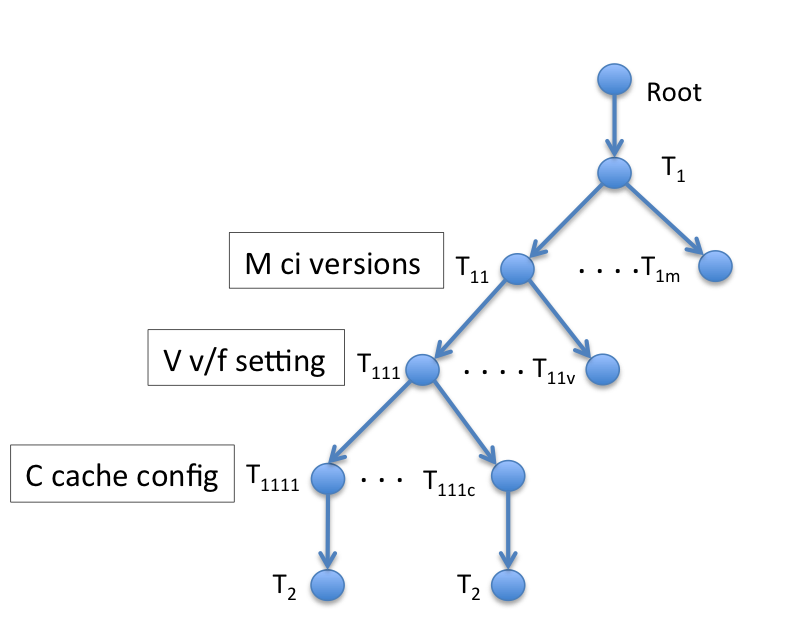
\includegraphics[width=0.36\textwidth]{branch.png}
\label{fig:bnb}
\caption {Example of Branching}
\end{figure}

The pseudo code for our branch and bound algorithm is shown in Algorithm
\ref{BnB}. Let $A_c$ and $P_c$ be the area and period constraints
provided as an input.
In each iteration, we map a task to one of the existing PEs (in lines
14-28) or to a new PE (in lines 30-45), and select a set of custom
instructions and voltage/frequency level for it. For a task $T_i$, the
algorithm enumerates all of its possible implementations which are the
combinations of sets of custom instructions, cache configurations and
voltage/frequency levels. And each of the customized versions are further
branched into multiple versions corresponding to different voltage/
frequency settings. For each of these versions, it could be mapped to
one of the already existing PEs or a new PE. And each PE can further
be tailored based on the various cache configuration supported. This
explains our branching technique in searching the entire design space
tree. In lines 19 and 35, the proceduce \textit{calculate\_params}
updates the current estimation of area, period and energy. In Figure
\ref{fig:bnb}, the number of existing PE for the first task $T_1$ is
null.

At level \textit{i} of the search tree, we have a partial solution
explaining the choice of configurations chosen for tasks $T_1,
T_2...T_i$, the voltage/frequency settings and the cache configuration
for each of the PEs already mapped. Let the period and area in the
partial solution space be \textit{period} and \textit{area} respectively.
With this partial solution, we can prune the subtree based on the
violation of any of the following constraints:

\begin{enumerate}
\item Pruning based on area constraint: By mapping only the software
only version of the remaining tasks in the existing PEs, the total area
occupied on-chip is still equal to \textit{area}. This is because the
software only version of the tasks does not occupy any extra area. If
this \textit{area} violates the area constraint, it is safe to prune the
entire subtree. For example, 

\item Pruning based on period constraint: By mapping the version of the
remaining tasks that has the minimal steady state execution time, the
lower bound of the new period can be estimated to be the \begin{math}
max(period_i, max(E_{i+1},..E_{N}))\end{math}. If the new period violates
the period contraint, it is safe to prune the entire subtree. For
example,

\item Pruning based on Lower Bound Cost (LBC): The LBC is defined as the
lowest possible energy consumption estimated at the level \textit{i}. For
each of the task, we identify the versions of the task that consume the
minimal energy. Then, the LBC can be estimated by summing the minimal
energy version of the remaining tasks $T_{i+1}, T_{i+2} ... T_{N}$. For
example, consider two tasks $T_i, T_j$ with the lowest steady state
energy consumption as $En_{ss,i}, En_{ss,j}$ respectively.
\begin{equation}
LBC = En_{ss,i} + En_{ss,j}
\end{equation}
The estimated LBC indirectly represents that the tasks are mapped to a
dedicated PE. If the more than one task is mapped to a single PE, the
energy consumed is definitely greater than or equal to the sum of the
steady state energy consumption of the individual tasks. If the tasks
$T_i, T_j$ were to be mapped in a single PE, then
\begin{equation}
\label{eq:lb}
LBC \leq En_{ss,i,j}
\end{equation}
From Equation \ref{eq:lb}, it is evident LBC estimated is indeed the
lowest possible energy acheivable in the subtree. One can easily prune a
subtree, if the existing best solution is smaller than the estimated LBC
for the energy.
\end{enumerate}


\begin{algorithm}
\caption{Branch and Bound algorithm}\label{BnB}
\begin{algorithmic}[1]
\State \begin{math} tasks = \lbrace T_1, T_2 ... T_N \rbrace \end{math};
\State $map = [ ]$; 
\State $currA = 0$; \Comment{current area}
\State $currP = 0$; \Comment{current period}
\State $currE = 0$; \Comment{current energy}
\State $existingPEs = \{\}$; \Comment{The set containing existing PEs}
\State
\State $BnB(tasks, A_c, P_c, map, existingPEs);$
\State
\Procedure{BnB}{$tasks, A_c, P_c, map, existingPEs$}
\State
\State $prune(tasks, A_c)$; \Comment{prunning based on the area}
\State $prune(tasks, P_c)$;\Comment{prunning based on the period}
\State $prune(tasks, best\_solution)$; \Comment{prunning based on the LBC}
\State
\If{$tasks \ne null$}  
\State $\backslash\ast$ mapping to one of the existing PEs $\ast\backslash$
\State T = remove a task from $tasks$;
\State
\For{j = 1 to M } \Comment{CIS versions}
\For{k = 1 to V } \Comment{V/F settings}
\For{ each PE in ex\_pe }
\State Add $T_{ijk}$ to map\{PE\};
\State $(currA, currP, currE)$=cal\_params(map($PE$));
\State
\If {$period \leq P_c$ \&\& $area \leq A_c$} 
\State $BnB(tasks, A_c, P_c, map, existingPEs)$;
\Else
\State update $(currA, currP, currE)$ to previous value;
\State Remove $T_{ijk}$ from map\{PE\};
\EndIf
\EndFor
\EndFor
\EndFor
\State
\State $\backslash\ast$ mapping to a new PE $\ast\backslash$
\For{j = 1 to M } \Comment{CIS versions}
\For{k = 1 to V } \Comment{V/F settings}
\For{l = 1 to C }  \Comment{C Cache Configs}
\State Add $T_{ijk}$ to map\{$PE_{l}$\};
\State Add $PE_{l}$ to $existingPEs$ ;
\State $(currA, currP, currE)$=cal\_params(map($PE_{l}$));
\State
\If {$period \leq P_c$ \&\& $area \leq A_c$} 
\State $BnB(tasks, A_c, P_c, map, existingPEs)$;
\Else
\State update $(currA, currP, currEn)$ to previous value;
\State Remove $T_{ijk}$ from map{$PE_{l}$};
\State Remove $PE_{l}$ from $existingPEs$;
\EndIf
\EndFor
\EndFor
\EndFor
\State

\Else 
\State $\backslash\ast$ We have a solution $\ast\backslash$
\State Update the best solution
 \EndIf
\State
\EndProcedure
\end{algorithmic}
\end{algorithm}
   

\section{Experimental Setup}
\label{sec:experiment}

We use a commercial tool set Xtensa RD-2011.2 from Tensilica Inc., \ref{}. Our base processor is Xtensa LX2 extensible cores and its configurations are summarized in Table \ref{tab:p_config}. The tool set includes C/C++ compiler that can compile C/C++ code for the target LX2 processor. The target application is simulated in the Instruction Set Simulator (ISS) that is included in the toolset. We use the Xtensa PRocessor Extension Synthesis (XPRES) compiler provided by the toolset to generate the various customized versions of the tasks. The newly generated task versions consist of any combination of fused operations, FLIX instructions, vector operations and specialized operations. 
%Figure \ref{} shows the performance vs area trade off for various customized versions of the tasks. 

In our experiments, we use five different instruction cache configurations ranging from 1 KB to 16 KB. Table \ref{tab:p_config} shows the area consumed by various cache configurations. We modify only instruction cache, but our technique can easily be extended to data cache too. We use Xt-Xenergy tool included in the toolset to measure both the dynamic and leakage energy consumptions. We use five different frequency levels ranging from 1.5 Ghz to 533 Mhz. We always set the voltage that supports the frequency being set ~\ref{}. We perform all our simulations at the maximum frequency and voltage. We estimate the power consumption at the frequency level $i$ using the following equation,
\begin{equation}
P_i = \frac{P_{max} * (V_i)^2 * F_i} {(V_{max})^2 * F_{max}}
\end{equation}  

We use popular streaming applications like MP3 encoder and JPEG encoder. Figure \ref{fig:benchmark} shows the various compute intensive kernels in the application. 

\begin{figure}[h]
\label{fig:benchmark}
\center
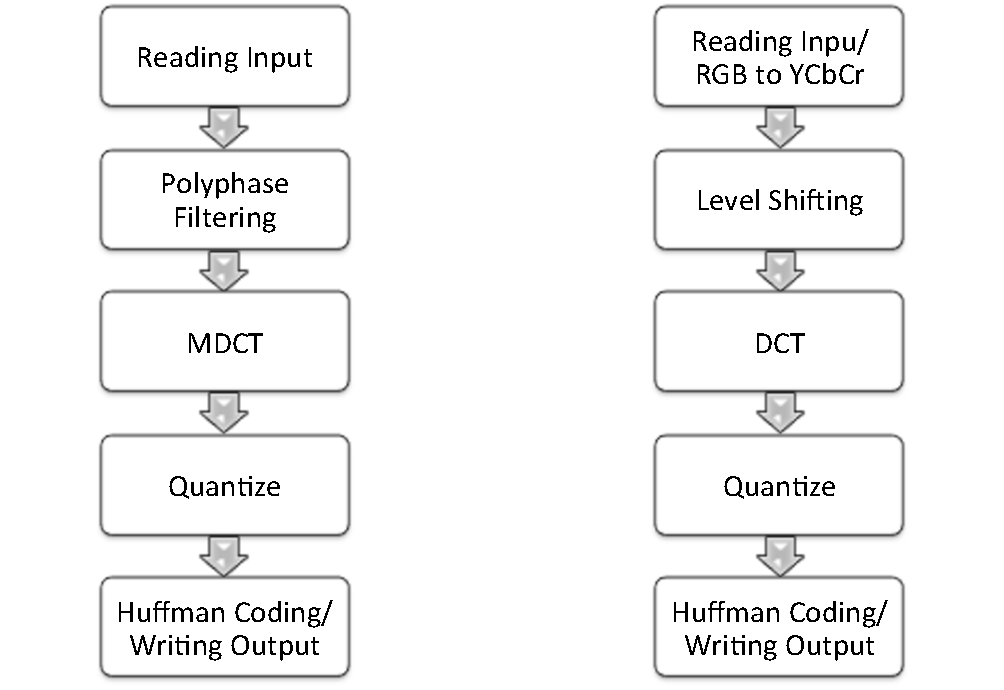
\includegraphics[width=0.40\textwidth, height=0.32\textwidth]{benchmark.pdf}
\label{fig:cache-size}
\caption {MP3 and JPEG}
\end{figure}

\begin{center}
\begin{table}
\begin{tabular}{|c|c|}
\hline
Frequency & 1.5 Ghz\ \\
\hline
Pipeline Depth & 5\ \\
\hline
Process Techology & 65nm GP \ \\
\hline
Core Area & 82806 gates or 0.451 $mm^2$\ \\
\hline
Max Instruction Width & 8 bytes\ \\
\hline
Data Cache size & 32 KB\ \\
\hline
Instruction Cache Size & 0.452 $mm^2$,\ \\
16K, 8K, 4K, 2K, 1K  & 0.275 $mm^2$, 0.174 $mm^2$,\ \\
 & 0.124 $mm^2$, 0.103 $mm^2$\ \\
\hline
I-Cache \& D-cache line size & 16 bytes\ \\
\hline
I-Cache \& D-cache Assoc & Direct mapped\ \\
\hline
PIF Interface & 32 bytes\ \\
\hline
Other Features & Boolean Registers, MUL32 \ \\ 
& and MAC16 instructions\ \\
& Functional unit clock gating,\ \\ 
& Flip-Flop register files\ \\
\hline
\end{tabular}
\caption{Baseline Processor Configuration.}
\label{tab:p_config}
\end{table}
\end{center}

\section{Results}
We verify the estimation of the steady state execution time and energy consumption from the stage \textit{latency/energy estimation} in our framework. Table \ref{tab:est} summarizes the accuracy of our estimation for the streaming applications JPEG and MP3. We varied the number of tasks mapped on a PE and compared our estimations with the actual simulation. 

\begin{table}
{
\label{tab:est}
\begin{tabular}{|c|c|c|c|c|c|}
\hline
Benchmark &  Number of &\multicolumn{2}{|c}{Execution} & \multicolumn{2}{|c|}{Energy} \ \\
& tasks mapped & \multicolumn{2}{|c|}{Time}& \multicolumn{2}{|c|}{Consumption}\ \\
\hline
& & Max & Avg & Max & Avg\ \\
& & error & error & error & error\ \\
& & (\%) &  (\%) &  (\%) &  (\%)\ \\
\hline
\multirow{5}{*}{JPEG} &  1 & & & & \ \\
& 2 & & & & \\
& 3 & & & & \\
& 4 & & & & \\
& 5 & & & & \\
\hline
\multirow{5}{*}{MP3} &  1 & & & & \ \\
& 2 & & & & \\
& 3 & & & & \\
& 4 & & & & \\
& 5 & & & & \\
\hline
\end{tabular}
}
\end{table}

\begin{center}
\begin{table*}[ht]
{
\begin{tabular}{|c|c|c|c|c|c|c|c|}
\hline
 &  &\multicolumn{3}{|c|}{\textbf{Hierarchical Approach}} &  \multicolumn{3}{|c|}{\textbf{Ci x Ca x DVFS}}\\
%\cline{3-9}
\hline
Benchmark&Experiment &Maximum&Minimum& Average&Maximum&Minimum& Average\\
& Number & Improvement & Improvement & Improvement & Improvement & Improvement & Improvement\\
& & (\%) & (\%) & (\%) & (\%) & (\%) & (\%)\\ 
\hline
\multirow{2}{*}{JPEG} & 1 & 29.51 & 1.27 & 24.35 & 32.31 & 3.27 & 26.52\ \\
& 2 & 29.04 & 2.23 & 26.31 & 29.04 & 0.532 & 25.12 \ \\
\hline
\multirow{2}{*}{MP3} & 1 & 41.78 & 3.27 & 43.02 & 49.01 & 10.49 & 44.17\ \\
& 2 & 43.03 & 6.78 & 39.08 & 47.30 & 12.50 & 43.97 \ \\
\hline
\end{tabular}
}
\hfill{}
\caption{Experimental results in comparison with \textbf{Ci+Ca}}
\label{tb:comparison}
\end{table*}
\end{center}

%\begin{figure}[h]
%\center
%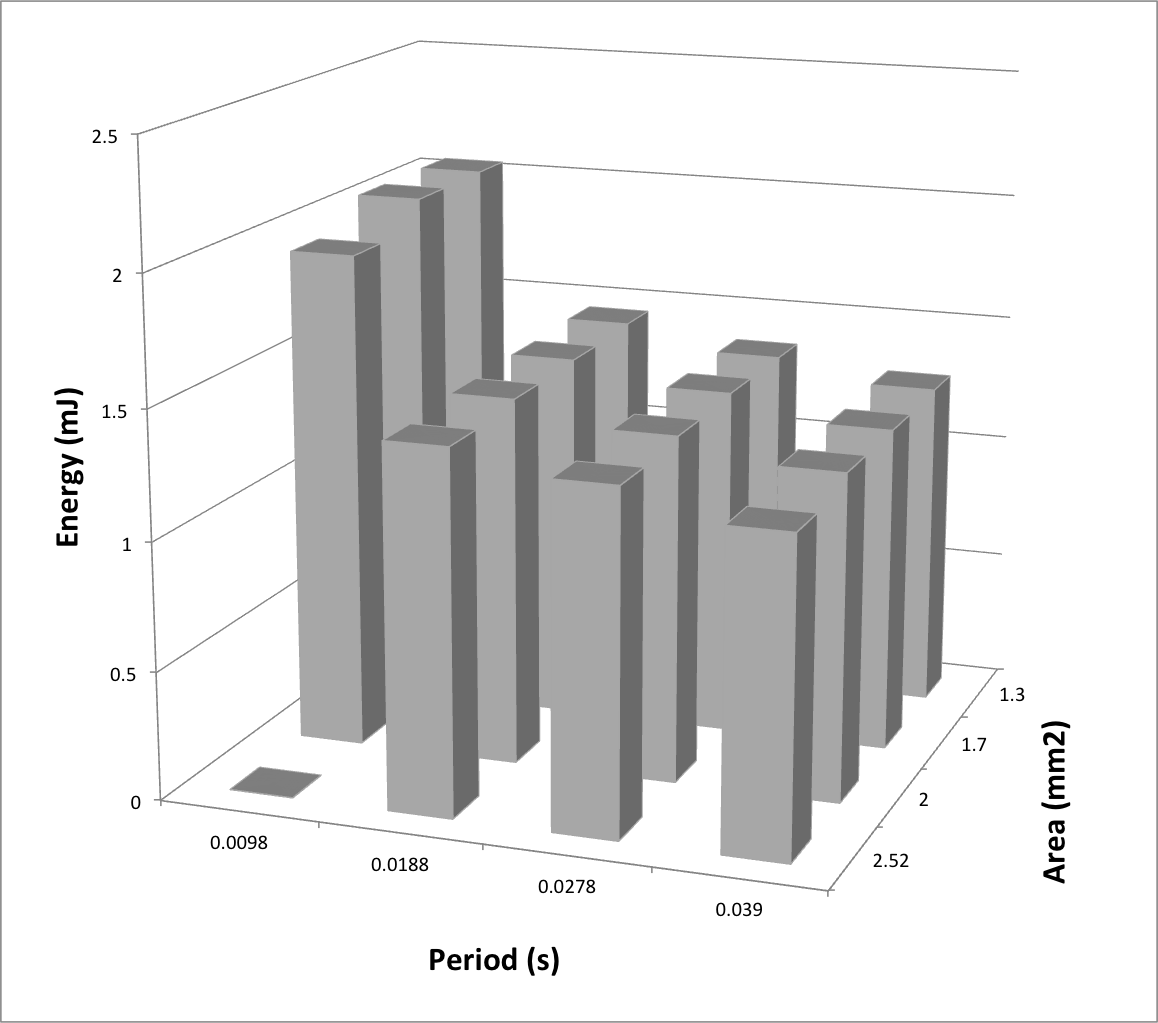
\includegraphics[width=0.36\textwidth]{CixCa+dvfs.png}
%\label{fig:CIxCa+dvfs}
%\caption {CixCa+DVFS for MP3}
%\end{figure}

%\begin{figure}[h]
%\center
%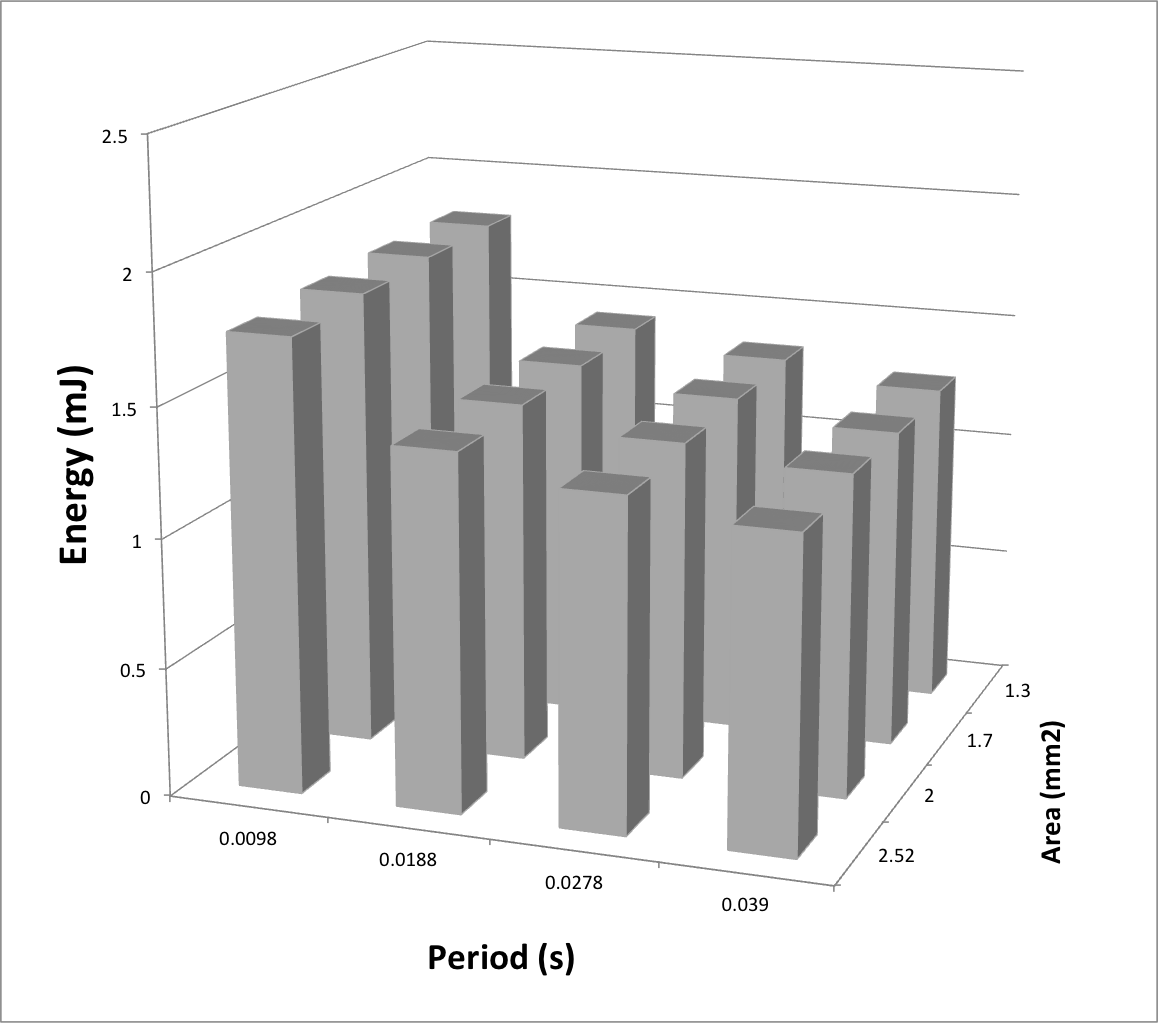
\includegraphics[width=0.36\textwidth]{CixCaxDVFS.png}
%\label{fig:CixCaxDVFS}
%\caption {CixCaxDVFS for MP3}
%\end{figure}
We compare the optimal points ASIP configuration obtained by the following techniques:
\begin{enumerate}
\item \textbf{CixCaxDVFS}: We use our branch and bound technique to find the optimal energy efficient ASIP configuration while modifying custom instruction set, cache configurations and voltage/frequency setting.
\item \textbf{CixCa+DVFS}: We call this technique as \textbf{Hierarchical Approach}. At the first stage, we optimize for the energy by only modifying custom instruction set and cache configurations. With the ASIP configuration obtained from the first stage, we apply different voltage/frequency setting to further reduce the energy. This technique can be derived by adding DVFS to the technique mentioned in \ref{}. 
\item \textbf{Ci+Ca}: Energy optimization by modifying only custom instruction set and cache configurations.
\end{enumerate}   

All the optimal points selected respects the input area and period constraints provided. As mentioned before, our design space consists of more than billion points along the axes of period, area and energy. Hence, it is not practical to plot all the points in a graph. Furthermore, we have two input constraints in terms of area and period. To get representative inputs for comparison, we perform two experiments per benchmark. In each of the experiments, we employ Latin hypercube sampling to generate 500 different tuples consisting of the area and period constraint. Using our branch and bound technique, we determine the lower bound of the period and the upper bound of the area by giving \textit{infinity} as an input constraint for both area and period for the target application. Similarly, the upper bound for the period is determined by summing the execution time of the software only versions of each task at the lowest possible cache configuration. The lowest bound for the area is equivalent to the size of a single PE and smallest cache configuration supported. With these bounds, latin hypercube sampling \ref{} efficiently covers the entire design space. 

We compare the results of the \textbf{CixCaxDVFS} and \textbf{CixCa+DVFS} with that of \textbf{Ci+Ca}. It is evident from the Table \ref{tb:comparison}, both the techniques significantly outperforms \textbf{Ci+Ca}. On an average, \textbf{CixCaxDVFS} performs better than \textbf{CixCa+DVFS}. This is because, the hierarchical nature of the technique \textbf{CixCa+DVFS} could result in the local optimum in comparison to the global optimum acheivable by \textbf{CixCaxDVFS}. Figure \ref{fig:CIxCa+dvfs} and \ref{fig:CIxCaxDVFS} shows the optimal energy acheivable for four different area and period constraint. In case of the hierarchical approach, we observed that there exists input constraints that was not satisfied to determine the optimal point. Thus, suggesting to consider all the three techniques (\textbf{Ci, Ca, DVFS} together. 

\section{Conclusion}





%
% The following two commands are all you need in the
% initial runs of your .tex file to
% produce the bibliography for the citations in your paper.
%\bibliographystyle{abbrv}
%\bibliography{sigproc}  % sigproc.bib is the name of the Bibliography in this case
% You must have a proper ".bib" file
%  and remember to run:
% latex bibtex latex latex
% to resolve all references
%
% ACM needs 'a single self-contained file'!
%
%APPENDICES are optional
%\balancecolumns

%\end{document}
%\scriptsize{
\bibliographystyle{plain}
\bibliography{bibl}
%}
\end{document}
